\documentclass[12pts,a4paper]{book}

\usepackage{lipsum}

<<<<<<< HEAD
=======
\usepackage[style = trad-abbrv, backend = bibtex, sorting = none, backref=true]{biblatex} %style = trad-abbrv
%		\addbibresource{06-Bibliografia/references.bib}
\addbibresource{references.bib}
>>>>>>> 65711adc10d96288917d1aaba2996bf656bbde5a
%!TeX root = ../main.tex

%-------------------------------------------------------------------------------
%                                   PACKAGES 		                                    |
%-------------------------------------------------------------------------------

%\usepackage{pslatex}						%Times New Roman font 
\usepackage{multicol}						% for pages with multiple text columns, e.g. References
	\setlength{\columnsep}{20pt} 				% space between columns; default 10pt quite narrow
\usepackage{multirow}
\usepackage{listings}                    		% Allows to add coding lines 
\usepackage{emptypage}						% Eliminates headers and footnotes in empty pages
\usepackage{makeidx}							% Add glosaries
%\usepackage[style=list,toc,number=none]{glossary}
\raggedbottom								% Makes LaTeX send tha white spaces to the background
\usepackage[bottom]{footmisc}					% for the footnotes; perpage -> inicia la numeración en la página misma
\usepackage{fancyhdr}						% for better header layout
\usepackage{eucal}
\usepackage{ifthen}
\usepackage[nottoc]{tocbibind} 				% correct page numbers for bib in TOC, nottoc suppresses an entry for TOC itself
%\usepackage{nextpage}
\usepackage{titlesec}
\usepackage{imakeidx}						% for indexes
\makeindex[intoc]
\usepackage{setspace}

\usepackage{enumitem}
\usepackage{etoolbox}
 % restart the enumerate list every chapter
 \preto\chapter{%
   \restartlist{enumerate}%
}

	%---------------------- Figures ----------------------------
		\usepackage[margin=10pt,font=scriptsize,labelfont=bf, ]{caption}  
		\usepackage[labelformat=simple]{subcaption} % labelformat=simple   O brace
%		\usepackage{subcaption}
%			\captionsetup[subfigure]{labelformat=simple}
		%\usepackage[bf,SL,BF]{subfigure}         
	    \usepackage{float}
		%	\floatsetup[subfigure]{style=plain,heightadjust=object,
		%					capbesideposition={left,top},
		%					capbesidesep=space}
			%\DeclareCaptionSubType[alph]{figure}
			%\captionsetup[subfigure]{labelformat=brace,justification=centerlast}
		\usepackage[export]{adjustbox}
		\usepackage{wrapfig}                    			% to include figure with text wrapping around it

	%--------------------- Color/equations -related stuff
		\usepackage{xcolor}
			%UNAM color palette
			\definecolor{UNAMblue}{RGB}{0,60,113}		% Blue pantone  541 (C)
			\definecolor{UNAMgold}{RGB}{234,221,150}		% Gold pantone  460  (C) ??

		\usepackage{empheq}
		\usepackage[most]{tcolorbox}
%			\tcbset{colback=lgreen,   colbacktitle = dgreen, frame hidden , % colframe= lgray,
%			fonttitle=\bfseries , boxrule = 0pt, standard jigsaw,  opacityback=.85, opacitybacktitle =1}% sharp corners = downhill, boxrule = .75mm }

	%----------------------- Language and references ------------------------------
		\usepackage[spanish,mexico]{babel}
		\usepackage[T1]{fontenc}			 		% 8-bits fonts
		\usepackage[utf8]{inputenc}           			% Complete latin alfabet: Accents and so on
		\spanishdecimal{.}
%		\usepackage[ square, comma, sort&compress, numbers]{natbib}
%											These are on the main.tex
		\usepackage[style = draft, backend = bibtex, sorting = none, backref=true]{biblatex} %style = trad-abbrv
		\addbibresource{0-Bibliografia/references.bib}
		 % The settings for the hyperref package are found below in the PDF/PS set up section 
		\addto\captionsspanish{\renewcommand{\figurename}{Fig.}}

	%------------------------- Maths --------------------------------------
		\usepackage{amssymb, amsmath, amsbsy, amsfonts}	% Math symbols and so on
		\usepackage{mathrsfs}						
		\usepackage{mathdots}                    			%  \iddots
		\usepackage{mathtools}
		\usepackage{physics}

	%------------------------- Tikz --------------------------------------
		\usepackage{tikz,pgfplots}
		\usetikzlibrary{hobby} 
			\usetikzlibrary{decorations.shapes}
			\usetikzlibrary{arrows.meta,calc,decorations.markings,math,arrows.meta}
			\usetikzlibrary{arrows,shapes,positioning}
			\usetikzlibrary{%
  							decorations.pathreplacing,%
						    decorations.pathmorphing%
							}	
			\usepackage{tikz-3dplot}
			%-------Dar dirección de las líneas (PONER FLECHITAS)
				\tikzstyle arrowstyle=[scale=1]
				\tikzstyle directed=[postaction={decorate,decoration={markings,
									 mark=at position .65 with{\arrow[arrowstyle]{stealth}}}}]
				\tikzstyle reverse directed=[postaction={decorate,decoration={markings,
									mark=at position .65 with {\arrowreversed[arrowstyle]{stealth};}}}]  		 
									
					

%------------------------- hyperref package --------------------------------------
   \usepackage[ pdftex, plainpages = false, pdfpagelabels, 
                 pdfpagelayout = OneColumn, % display single page, advancing flips the page - Sasa Tomic
                 bookmarks,
                 bookmarksopen = true,
                 bookmarksnumbered = true,
                 breaklinks = true,
                 linktocpage,
%                 pagebackref,
                 colorlinks = true,
                 linkcolor = blue,
                 urlcolor  = blue,
                 citecolor = magenta,
                 anchorcolor = green,
				hyperfootnotes = true,
                 hyperindex = true,
                 hyperfigures
                 ]{hyperref} 
    \usepackage{graphicx}   %Used this insetad of  \usepackage[pdftex]{graphicx} 'cause it wasn't debugging. Don't know why
    \DeclareGraphicsExtensions{.png, .jpg, .pdf}

    \pdfcompresslevel=9




\title{Solución de Mie}
\author{Urrutia Anguiano, Jonathan Alexis\\ Rojas, Isabel}

% ---------------------------For graphics / images
\usepackage{graphicx}
\graphicspath{{graphics/}}

\makeindex

\begin{document}
	\frontmatter
	
%	\blankpage
%	r.3 full title page
	\maketitle
%	r.5 contents
	\tableofcontents
%	\listoffigures
%	\listoftables

	\cleardoublepage
%\chapter*{Introduction}
%
%Aquí iría el texto que todos vamos a escribir al final, en donde hablamos del propósito del libro y esas cosas. Esto lod dejaremos al final.


% Start the main matter (normal chapters)
\mainmatter


\chapter{Repaso de electromagnetismo}
\label{ch:repasoEM} %-------------------Labels para los capítulos -> ch:LABEL

<<<<<<< HEAD
	El contenido propuesto es

	\begin{itemize}
	 \item Ecuaciones de Maxwell
	 \item Considerar la Ec. de Helmholts
	 \item Hablar sobre los campos EM armónicos
	 \item Vector de Poynting
	 \item Condiciones a la frontera de forma general
	 \item Condiciones a la frontera considerando una esfera
	\end{itemize}
=======
Con el propósito de desarrollar la solución de Mie, se comenzará por una breve revisión de algunos conceptos fundamentales del electromagnetismo. De esta forma, se establecerán las convenciones que serán usadas a lo largo de estas notas y, además, servirá como un punto de partida para el desarrollo del problema de esparcimiento.

\section{Ecuaciones de Maxwell}

Los fenómenos electromagnéticos son descritos casi por completo a través un conjunto de cuatro ecuaciones conocidas como \textit{ecuaciones de Maxwell}. Con ellas se determina el comportamiento y la propagación de los campos electromagnéticos y cómo son influenciados por fuentes externas~\cite{Jackson}. En el caso donde los campos eléctrico $\vb{E}$ y magnético $\vb{B}$ se propagan en el vacío las ecuaciones de Maxwell se escriben como~\cite{Jackson}:
%
	\begin{tcolorbox}[title = Ecuaciones de Maxwell en el vacío]\vspace*{-0.3cm}
\begin{flalign}
	&  & \div \vb{E} &= \frac{\rho_{tot}}{\epsilon_{0}}, &  & \text{Ley de Gauss eléctrica} \label{eq:maxwell1}\\
	&  & \div \vb{B} &= 0, &  & \text{Ley de Gauss magnética} \label{eq:maxwell2}\\
	&  & \curl \vb{E} &= - \pdv{\vb{B}}{t}, &  & \text{Ley de Faraday--Lenz} \label{eq:maxwell3}\\
	&  & \curl \vb{B} &= \mu_{0} \vb{J}_{tot}+ \epsilon_{0} \mu_{0} \pdv{\vb{E}}{t}, &  & \text{Ley de Amp\`ere--Maxwell}\label{eq:maxwell4}
\end{flalign}
\end{tcolorbox}
%
\noindent en donde $\epsilon_{0}$ es la permitividad eléctrica del vacío, mientras que $\mu_{0}$ es la permeabilidad magnética del vacío; $\rho_{total}$ se refiere a la densidad volumétrica de carga total y $\vb{J}_{tot}$ a la densidad volumétrica de corriente total. Es importante destacar que las Ecs.~\eqref{eq:maxwell1}--\eqref{eq:maxwell4} están escritas en unidades del sistema internacional. Cada una representa una expresión matemática que describe observaciones experimentales. No pueden ser demostradas pero su aplicabilidad es verificable, por ello, las ecuaciones de Maxwell se utilizan en diversos problemas que involucren sistemas macroscópicos~\cite{Reitz}.

Las Ecs.~\eqref{eq:maxwell1} y.~\eqref{eq:maxwell4} cambian su forma cuando los campos electromagnéticos se propagan en medios materiales. Para ello, es necesario considerar al vector de desplazamiento, definido como~\cite{Jackson}:
\begin{equation}
\vb{D} = \epsilon_{0} \vb{E} + \vb{P},
\label{eq:vecDes}
\end{equation}
con $\vb{P}$ la polarización del material, y al campo $\vb{H}$, cuya relación con el campo magnético es~\cite{Griffiths}:
\begin{equation}
\vb{H} = \frac{\vb{B}}{\mu_{0}}-\vb{M}.
\label{eq:campoH}
\end{equation}
donde $\vb{M}$ corresponde a la magnetización del medio material. Por tanto, las ecuaciones de Maxwell en medios materiales son~\cite{Jackson}:
\begin{tcolorbox}[title = Ecuaciones de Maxwell en medios materiales]\vspace*{-0.3cm}
\begin{subequations}
	\begin{align}
		\div \vb{D}& = \rho_{ext},\label{eq:maxwell1_mat}\\
		\div \vb{B}& =0,\\
		\curl \vb{E}& = - \pdv{\vb{B}}{t},\\
		\curl \vb{H} &= \vb{J}_{ext} + \pdv{\vb{D}}{t},
		\label{eq:maxwell4_mat}
	\end{align}
\end{subequations}
\end{tcolorbox}
\noindent en donde $\rho_{ext}$ corresponde a la densidad de carga volumétrica externa y $\vb{J}_{ext}$ es la densidad de corriente volumétrica externa. 

Las ecuaciones de Maxwell en para medios materiales  [Ecs.~\eqref{eq:maxwell1_mat}--\eqref{eq:maxwell4_mat} contienen la información del material a través de dos cantidades conocidas como polarización, $\vb{P}$, y magnetización, $\vb{M}$~\cite{Griffiths}. Por ello, es preciso contar con relaciones que describan el comportamiento de los materiales bajo la influencia del campos EMs. En general, la polarización y magnetización no se pueden describir en una forma reducida y simple. Sin embargo, pueden realizarse algunas suposiciones sobre el material en cuestión. El caso más sencillo consiste en un medio material que cumple con ser \textit{homogéneo} (sus propiedades son iguales en cada punto), \textit{isotrópo} (sus propiedades ópticas en cada punto son independientes de la dirección) y tiene una respuesta ante los campos EMs de tipo \textit{lineal}. Dichas características permiten escribir \textit{relaciones constitutivas} que establecen una relación entre los cuatro campos vectoriales $\vb{E}$, $\vb{B}$, $\vb{D}$ y $\vb{H}$, La polarización y la magnetización cumplen con~\cite{Griffiths}:
%
\begin{eqnarray}
	\vb{P}=\epsilon_{0}\chi_{e}\vb{E},\qquad \vb{M}=\chi_{m}\vb{H},\label{eq:rel_constitutivas}
\end{eqnarray} 
%
respectivamente, donde se ha utilizado que $\chi_{e}$ ($\chi_{m}$) es la susceptibilidad eléctrica (magnética). De está forma, al sustituir las Ecs.~\eqref{eq:rel_constitutivas} en las expresiones para los campos $\vb{D}$ [Ec.~\eqref{eq:vecDes}] y $\vb{H}$ [Ec.~\eqref{eq:campoH}], se llega a~\cite{Griffiths}
\begin{eqnarray}
	\vb{D}=\epsilon\vb{E}, \qquad \text{y} \qquad
	\vb{H}=\frac{1}{\mu} \vb{B}, \label{eq:hache}
\end{eqnarray}
donde  $\epsilon\equiv\epsilon_{0}\left(1+\chi_{e}\right)$ y $\mu\equiv\mu_{0}\left(1+\chi_{m}\right)$ son la permitividad y permeabilidad características del medio material, respectivamente. En general, $\epsilon$ es una cantidad compleja que depende de la frecuencia de la onda incidente. A partir de ambas propiedades se expresa el índice de refracción del material en cuestión~\cite{Griffiths}
%
\begin{equation}
	n\equiv\sqrt{\frac{\epsilon\mu}{\epsilon_{0}\mu_{0}}}.
\end{equation}

\section{Condiciones a la frontera}
Las ecuaciones de Maxwell son ecuaciones diferenciales aplicadas localmente en cada punto del espacio~\cite{Jackson}. EN particular, es interesante conocer lo que sucede con las componentes de los campos $\vb{E}$, $\vb{B}$, $\vb{D}$ y $\vb{H}$ en la interfaz que separa dos medios. Para ello se inicia escribiendo a las ecuaciones de Maxwell en su forma integral~\cite{Griffiths}
\begin{subequations}
	\begin{align}
		\oint_{S}\vb{D}\cdot\dd{\vb{a}}&=Q_{tot},\label{MaxwellInt1}\\
		\oint_{S}\vb{B}\cdot\dd{\vb{a}}&=0,\label{MaxwellInt2}\\
		\oint_{P}\vb{E}\cdot\dd{\vb{l}} &=- \dv{}{t}\int_{S}\vb{B}\cdot\dd{\vb{a}},\label{MaxwellInt3}\\
		\oint_{P}\vb{H}\cdot\dd{\vb{l}}&=I_{tot}+\dv{}{t}\int_{S}\vb{D}\cdot\dd{\vb{a}}\label{eq:MaxwellInt4},
	\end{align}
\end{subequations}

Con el propósito de derivar estudiar la continuidad de los campos en una interfaz, primero, se suponen dos medios, cada uno caracterizado por sus propiedades ópticas: $\epsilon_{1},\:\mu_{1}$ para el medio 1 y $\epsilon_{2},\:\mu_{2}$ para el medio 2. La interfaz que separa ambos medios tiene densidad superficial de carga $\sigma_{tot}$ y una densidad superficial de corriente $\vb{K}_{tot}$. En particular, para analizar las componentes de $\vb{D}$ ortogonales a la interfaz, se realiza la integral en la Ec.~\eqref{MaxwellInt1}. Para ello, se elige un prisma rectangular como el que se muestra en la Fig.~\ref{fig:BoundaryConditions}(a) (conocido como \textit{Gaussian pillbox}); se supondra que su altura es $\delta$ y que sus caras paralelas a la superficie tienen un área $A$. Una parte del volumen estará por encima de la interfaz y el resto se encontrará por debajo. El vector normal a la superficie está denotado por $\vu{n}$. Puesto que la integral en la Ec.~\eqref{MaxwellInt1} es de superficie, se realiza sobre todas las caras del volumen. Sin embargo, se considera que la altura de la caja es infinitesimalmente pequeña ($\delta\to 0$). Por tanto, sólo las caras de área $A$ contribuyen, dando como resultado~\cite{Griffiths}: 
\begin{equation}
\begin{split}
\oint_{S}\vb{D}\cdot\dd{\vb{a}}=\left(D_{1}^{\perp}-D_{2}^{\perp}\right)A=Q_{enc},\label{eq:int1}
\end{split}
\end{equation}
donde $D_{1}\perp$ y $D_{2}^{\perp}$ corresponden a las componentes del vector de desplazamiento ortogonales a la interfaz en los medios 1 y 2, respectivamente. Ademas, $Q_{enc}$ es la carga encerrada por el volumen de la caja. Recordando que $Q_{enc}=\sigma_{enc}A$, se puede reescribir a la Ec.~\eqref{eq:int1} en términos de la densidad de carga superficial:
\begin{equation}
D_{1}^{\perp}-D_{2}^{\perp}=\sigma_{tot}.
\end{equation}
Por tanto, la componente perpendicular del campo $\vb{D}$ es discontinua en la frontera entre dos medios.
%\begin{equation}
%	\vb{D}_{1}\cdot \vb{A}-\vb{D}_{2}\cdot \vb{A}=\sigma_{tot}A
%\end{equation}
A través de un procedimiento similar y usando la Ec.~\eqref{MaxwellInt2}, se deduce que~\cite{Griffiths}
\begin{equation}
B_{1}^{\perp}-B_{2}^{\perp}=0,
\end{equation}
donde $B_{i}^{\perp}$ denota la componente del campo $\vb{B}$ perpendicular a la interfaz dentro del medio $i=1,\:2$. Es decir, la componente perpendicular del campo $\vb{B}$ es continua a través de la frontera.

Por otro lado, a partir de la Ec.~\eqref{MaxwellInt3} es posible describir la continuidad de las componentes del campo eléctrico paralelas a la interfaz. Con ese fin, la integral de trayectoria en la Ec.~\eqref{MaxwellInt3} se calcula utilizando un circuito rectangular como el mostrado en la Fig.~\ref{fig:BoundaryConditions}(b); su altura  es $\delta$ y el ancho $l$. Nuevamente, la mitad del circuito se encuentra inmerso en el medio 1 (sobre la interfaz) y el resto en el medio 2 (debajo de la interfaz). Se considerará el límite $\delta\to0$, por tanto, la integral queda como
\begin{equation}
\oint_{P}\vb{E}\cdot\dd{\vb{l}}=(E_{1}^{\parallel}-E_{2}^{\parallel})l=\vb{E}_{1}\cdot\vb{l}-\vb{E}_{2}\cdot\vb{l},
\end{equation}
siendo $E_{1}^{\parallel}$ y $E_{2}^{\parallel}$ las componentes del campo eléctrico paralelas a la superficie de la interfaz en los medios 1 y 2, respectivamente. Por otra parte, al considerar que la altura del circuito es infinitamente pequeña la contribución del campo magnético a la Ec.~\eqref{MaxwellInt3} es despreciable. Esto último puede entenderse al considerar que la integral de superficie del campo $\vb{B}$ da como resultado $B_{\perp}A^{*}$, con $A^{*}$ el área del circuito. Al realizar el límite $\delta\to0$, el área también tiende a cero. Por tanto, se concluye que~\cite{Griffiths}
\begin{equation}
\vb{E}^{\parallel}_{1}-\vb{E}^{\parallel}_{2}=\vb{0},
\end{equation}
es decir, los componentes del campo eléctrico paralelas a la interfaz son continuas sobre la frontera. 

De la Ec.~\eqref{eq:MaxwellInt4} se deduce una relación para las componentes del campo $\vb{H}$. Utilizando el circuito ya descrito, se realiza la integral de contorno~\cite{Griffiths}:
\begin{equation}
\oint_{S}\vb{H}\cdot\dd{\vb{l}}=(H^{\parallel}_{1}-H^{\parallel}_{2})l=\vb{H}^{\parallel}_{1}\cdot\vb{l}-\vb{H}^{\parallel}_{2}\cdot\vb{l},
\end{equation}
donde $H_{1}^{\parallel}$ y $H_{2}^{\parallel}$ son las componentes del campo eléctrico paralelas a la superficie de la interfaz en los medios 1 y 2, respectivamente. Se debe notar que la contribución del campo $\vb{D}$ a la Ec.~\eqref{eq:MaxwellInt4} es despreciable debido a que, al considerar $\delta\to0$, el área del circuito es infitesimalmente pequeña. Por otra parte, la corriente encerrada por el circuito es
$I_{enc}$. Puesto que para este caso sólo la densidad de corriente superficial contribuye, la corriente se escribe como~\cite{Griffiths}: 
\begin{equation}
I_{tot}=\vb{K}_{tot}\cdot\left(\vu{n}\times\vb{l}\right)=\left(\vb{K}_{tot}\times\vu{n}\right)\cdot \vb{l} 
\end{equation}
donde, $\vu{n}$ es un vector unitario y normal a la interfaz. De esta forma, se llega a que~\cite{Griffiths}
\begin{equation}
\vb{H}_{1}^{\parallel}-\vb{H}^{\parallel}_{2}=\vb{K}_{tot}\times\vu{n}.
\end{equation}
Las componentes paralelas de $\vb{H}$ son discontinuas en la frontera por una cantidad proporcional a la densidad de corriente superficial.
\begin{figure}[ht!]
	\centering
	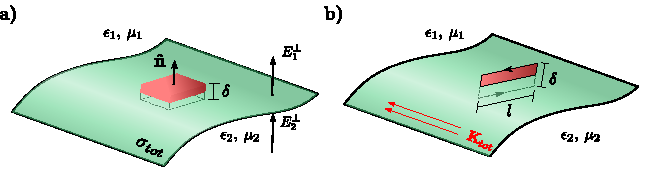
\includegraphics[width=12.5cm]{1-Capitulo-Repaso/0-Diagramas/dibujo.pdf}
	\caption[Condiciones de frontera]{Diagrama de una interfaz (superficie en verde) que separa dos medios distintos. El \textit{medio 1} tiene propiedades ópticas $\epsilon_{1},\,\mu_{1}$, mientras que las del \textit{medio 2} son $\epsilon_{2},\,\mu_{2}$. \textbf{a)} Prisma rectangular con altura $\delta$ y cuyas caras paralelas a la superficie tiene un área $A$. Sobre la superficie que separa a los medios hay una densidad de carga superficial total igual a $\sigma_{tot}$. \textbf{b)} Circuito rectancular con altura $\delta$ y ancho $l$. En la interfaz entre los medios hay una densidad de corriente superficial $\vb{K}_{tot}$.}
	\label{fig:BoundaryConditions} 
\end{figure}
% 
En particular, cuando los medios son lineales, las condiciones de frontera son~\cite{Griffiths}:
\begin{tcolorbox}[title = Condiciones de frontera para materiales lineales]
\begin{equation}
\begin{aligned}
&\epsilon_{1}E_{1}^{\perp}-\epsilon_{2}E_{2}^{\perp}=\sigma_{tot},&\qquad&\vb{E}_{1}^{\parallel}-\vb{E}_{2}^{\parallel}=\vb{0},\\[2pt]
&B_{1}^{\perp}-B_{2}^{\perp}=0,&\qquad& \frac{1}{\mu_{1}}\vb{B}^{\parallel}_{1}-\frac{1}{\mu_{2}}\vb{B}^{\parallel}_{2}=\vb{K}_{tot}\times\vu{n},
\end{aligned}\label{eq:Condiciones_fronteras_lineal}
\end{equation}
\end{tcolorbox}
En las Ecs.~\eqref{eq:Condiciones_fronteras_lineal} es posible notar que, si no hay fuentes externas, tanto componentes paralelas como perpendiculares de los campos EMs son continuas en la frontera entre ambos medios.

\section{Campos eléctromagnéticos armónicos}
Las ecuaciones de Maxwell imponen relaciones entre los cuatro campos $\vb{E}$, $\vb{B}$, $\vb{D}$ y $\vb{H}$. Es posible desacoplar a las ecuaciones de Maxwell y obtener una ecuación para sólo uno de los campos. Para ello, primero, se observa que, en el vacío y sin fuentes externas, es decir, $J_{tot},\:\rho_{tot}=0$, se cumple que
\begin{eqnarray}
	\vb{D}=\epsilon_{0}\vb{E},\qquad\text{y}\qquad\vb{H}=\frac{\vb{B}}{\mu_{0}},
\end{eqnarray}
Por otro lado, se calcula el rotacional de la Ec.~\eqref{eq:maxwell4_mat}
\begin{equation}
	\curl \curl \vb{H}= - \laplacian \vb{H}= \pdv{\curl\vb{D}}{t},\label{eq:1}
\end{equation}
donde se utilizó la relación~\cite{Griffiths}
\begin{equation}
\curl\curl\vb{A}= \grad(\div \vb{A}) - \laplacian \vb{A},\label{eq:propiedad}
\end{equation}
y que $\div \vb{H}=0$. Además, se cumple también que $\curl\vb{D}=-\epsilon_{0}\mu_{0}\pdv{\vb{H}}{t}$. Por tanto, sustituyendo en la Ec.~\eqref{eq:1}, se obtiene que~\cite{Griffiths}
\begin{equation}
\laplacian{\vb{H}}+\epsilon_{0}\mu_{0}\pdv[2]{\vb{H}}{t}=0,\label{eq:ecuacion_de_onda_H}
\end{equation}
A través de un procedimiento análogo se llega a
\begin{equation}
		\laplacian{\vb{E}}+\epsilon_{0}\mu_{0}\pdv[2]{\vb{E}}{t}=0, \label{eq:ecuacion_de_onda_E}
\end{equation}
Las Ecs.~\eqref{eq:ecuacion_de_onda_H} y~\eqref{eq:ecuacion_de_onda_E} son la ecuación de onda vectorial para el campo $\vb{H}$ y $\vb{E}$, respectivamente. Cada una de las componentes de los campos EMs cumplen la ecuación de onda escalar en un medio homogéneo, libre de corrientes y cargas~\cite{BornWolf1980}:
\begin{equation}
	\laplacian V-\frac{1}{c^{2}}\pdv[2]{V}{t}=0,
\end{equation}
en donde $c=1/\sqrt{\epsilon_{0}\mu_{0}}$ corresponde a la velocidad de la luz.

Una de las soluciones más sencillas a la ecuación de onda escalar está dada por~\cite{Griffiths}
\begin{equation}
	V=Ae^{i\left(\vb{k}\cdot\vb{r}-\omega t\right)},\label{eq:funcion_onda}
\end{equation}
donde $\vb{k}$ es el vector de onda, asociado a la dirección de propagación de la onda, y $\omega$ es la frecuencia angular, da el número de vibraciones en $2\pi$ segundos~\cite{BornWolf1980}. La amplitud $A$ es una cantidad compleja. La Ec.~\eqref{eq:funcion_onda} también pudo ser escrita en términos de las funciones seno y coseno, sin embargo, es preferible el uso de exponenciales complejas puesto que es más sencillo de manipular para hacer cálculos. Al final, sólo se considera la parte real de la función de onda~\cite{Griffiths}. A partir de la Ec.~\eqref{eq:funcion_onda} se distingue a la onda plana; se obtiene cuando $\vb{k}\cdot\vb{r}$ es constante, por tanto, en cada instante de tiempo $V$ es constante en cada plano definido por $\vb{k}\cdot\vb{r}$~\cite{Griffiths}. 

Debido a la forma de la dependencia temporal en la Ec.~\eqref{eq:funcion_onda} se dice que el campo es armónico en el tiempo. Por ello, los campos EMs armónicos se escriben como~\cite{Griffiths}
%
\begin{eqnarray}
	\vb{E}_{c}=\vb{E}_{0}e^{i\left(\vb{k}\cdot\vb{r}-\omega t\right)},&&\vb{H}_{c}=\vb{H}_{0}e^{i\left(\vb{k}\cdot\vb{r}-\omega t\right)},\label{eq:Campos_armo}
\end{eqnarray}
con $\omega=kc$. En ausencia de fuentes externas los campos $\vb{E}$ y $\vb{H}$ son ortogonales entre sí y respecto al vector de onda $\vb{k}$, ver Fig.~\ref{fig:EHFields}. Se relacionan entre sí a través de la siguiente ecuación~\cite{Griffiths}:
\begin{equation}
	\vb{H}=\sqrt{\frac{\epsilon_{0}}{\mu_{0}}}\vb{k}\times\vb{E},
\end{equation}

Debido a la forma de los campos EMs [Ecs.~\eqref{eq:Campos_armo}], las ecuaciones de Maxwell se reescriben como~\cite{Bohren}
\begin{equation}
\div \epsilon \vb{E}_{c} = 0, 
\label{eq:maxwell1H}
\end{equation}
\begin{equation}
\div \vb{H}_{c} = 0, 
\label{eq:maxwell2H}
\end{equation}
\begin{equation}
\curl \vb{E_{c}} = i \omega \mu \vb{H}_{c}, 
\label{eq:maxwell3H}
\end{equation}
\begin{equation}
\curl \vb{H}_{c} = -i\omega \epsilon \vb{E}_{c}.
\label{eq:maxwell4H}
\end{equation}
Nuevamente, es posible desacoplar las ecuaciones de Maxwell. Para ello calculamos el rotacional de las Ecs. \eqref{eq:maxwell3H} y \eqref{eq:maxwell4H}:
\begin{equation}
\curl (\curl \vb{E})=i\omega \mu \curl \vb{H} = \omega ^{2} \epsilon \mu \vb{E},
\label{eq:curlE}
\end{equation}
\begin{equation}
\curl (\curl \vb{H})=-i\omega \epsilon \curl \vb{E} = \omega ^{2} \epsilon \mu \vb{H}
\label{eq:curlH}
\end{equation}
Usando la propiedad en la Ec.~\eqref{eq:propiedad}, se reescriben a las Ecs. \eqref{eq:curlE} y \eqref{eq:curlH} como sigue

\begin{tcolorbox}[title = Ecuación vectorial de Helmholtz]\vspace*{-0.3cm}
\begin{subequations}
	\begin{align}
\laplacian \vb{E} + \omega^{2} \epsilon \mu \vb{E}&=0, \label{eq:HelmholtzE}\\
\laplacian \vb{H} + \omega^{2} \epsilon \mu \vb{H}&=0,\label{eq:HelmholtzH}
	\end{align}
\end{subequations}
\end{tcolorbox}
\noindent en donde $k^{2}=\omega^{2} \epsilon \mu$.

\begin{figure}
	\centering
	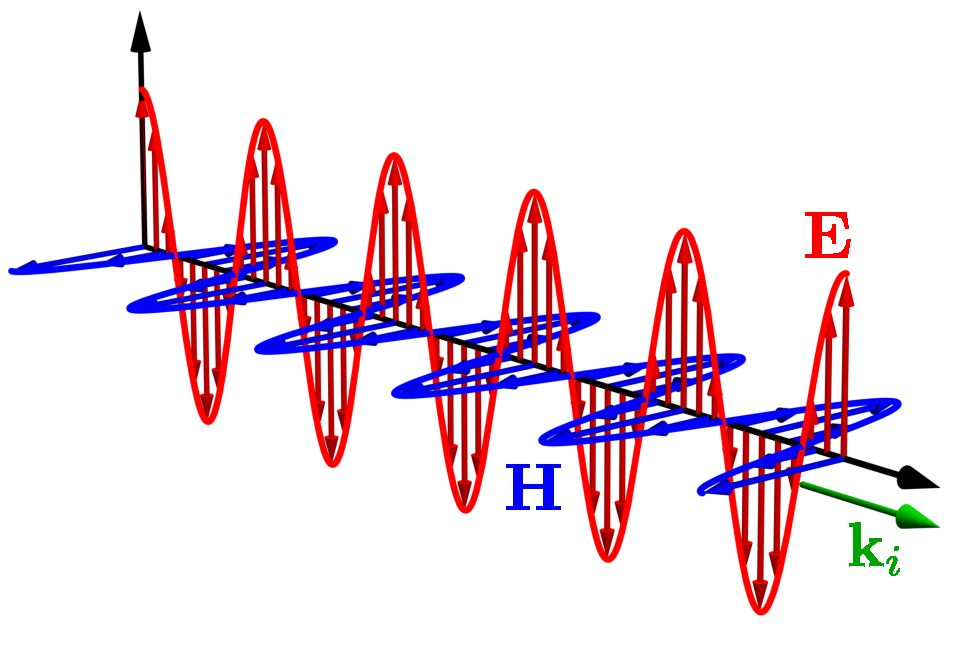
\includegraphics[width=9cm]{1-Capitulo-Repaso/0-Diagramas/campos.pdf}\vspace*{-0.3cm}
	\caption[Campo eléctromagnetico armónico]{Representación de los campos EMs armónico. En rojo se encuentra el campo eléctrico $\vb{E}$ y en azul el campo $\vb{H}$, para cada uno, las flechas indican la orientación de su oscilación. La flecha verde indica la dirección de propagación de la onda, dada por $\vb{k}_{i}$.}\label{fig:EHFields}
\end{figure}
\section{Vector de Poynting}

El vector de Poynting es una cantidad que indica la energía por unidad de tiempo, por unidad de área, transportada por los campos EMs, de forma general, se define como~\cite{Griffiths}:
\begin{equation}
\vb{S}=\left(\vb{E} \cross \vb{H}\right).
\label{eq:poynting}
\end{equation}
La energía por unidad de tiempo que cruza una superficie infinitesimal $\dd{\vb{a}}$ es $\vb{S}\cdot\dd{\vb{a}}$, y es llamado flujo de energía~\cite{Griffiths}.

En el caso de la luz, las longitudes de onda son tan cortas ($\sim 5\times10^{-7}$ m), y el periodo ($\sim10^{-15}$ s), que las mediciones macroscópicas involucran muchos ciclos, por ello no es viable medir directamente al vector de Poynting. Se utiliza el promedio temporal, denotado con $\expval{\quad}$~\cite{Griffiths}. Retomando el caso de campos EMs armónicos, el vector de Poynting luce de la siguiente forma
\begin{equation}
\vb{S} = \Re{\vb{E}_{c}} \cross \Re{\vb{H}_{c}},
\end{equation}
cuyo promedio temporal es~\cite{BornWolf1980}
\begin{equation}
\expval{\vb{S}}=\frac{1}{2}\left(\vb{E}_{c} \cross \vb{H}_{c}^{*}\right),
\label{eq:poynting_promedio}
\end{equation}
en donde $^{*}$ indica el complejo conjugado. El cálculo del promedio temporal se realiza sobre un ciclo completo. Ahora es posible calcular la potencia promedio por unidad de área transportada por una onda EM, es decir, la intensidad~\cite{Griffiths}
\begin{equation}
	I=\expval{S}
\end{equation}

Con el vector de Poynting también se determina la magnitud y dirección de la tasa de transferencia de energía electromagnética en cualquier punto del espacio \cite{Bohren}. Es posible cuantificar la tasa neta con la que la energía EM cruza la frontera de una superficie cerrada $A$ que encierra un volumen $V$~\cite{Bohren}:
\begin{equation}
W=- \int_{A} \vb{S} \vdot \vu{n} \dd A,
\label{eq:rateElecEnergy}
\end{equation}
donde $\vu{n}$ es el vector unitario normal a la superficie. Es importante notar que se agrega un signo menos en la Ec. \eqref{eq:rateElecEnergy} puesto que se ha elegido el vector normal que apunta hacia afuera del volumen. Entonces, si $\vb{S}$ es tal que apunta en la dirección contraria a $\vu{n}$, W será positiva. Lo cual indica que la energía se absorbe. 





%Esta parte corresponde a \textbf{Isabel}. El contenido propuesto es

%\begin{itemize}
% \item Ecuaciones de Maxwell
% \item Considerar la Ec. de Helmholts
% \item Hablar sobre los campos EM armónicos
% \item Vector de Poynting
% \item Condiciones a la frontera de forma general
% \item Condiciones a la frontera considerando una esfera
%\end{itemize}
>>>>>>> 65711adc10d96288917d1aaba2996bf656bbde5a

\chapter{Teoría general de esprcimiento}
\label{ch:EsparcimientoGral}

	El contenido propuesto es

	\begin{itemize}
	 \item Matriz de esparcimiento general
	 \item Teorema óptico
	\end{itemize}

\chapter{Los armónicos esféricos vectoriales}
\label{ch:ArmonicosEsferico} 
	%Esta parte corresponde a \textbf{Jonathan}. El contenido propuesto es
	%
	%\begin{itemize}
	% \item Propuesta de M y N (gral)
	% \item Función generadora (gral)
	% \item Geometría esférica para M y N
	% \item Geometría esférica para M y N -- Relaciones de ortogonalidad
	%  \item Descomposición de una onda plana en la base de los AEV
	%\end{itemize}
%!TeX root = ../main.tex

Para encontrar una solución al problema de esparcimiento y absorción de la luz por una partícula esférica, se considerará una región del espacio libre de fuentes y que los campos EM son armónicos en el tiempo, como se presentan en las Ecs. \eqref{} {\color{red} Isabel, pondrás las ecuaciones de Maxwell con su transformada de Fourier?}. Asimismo, se plantea un base de funciones vectoriales que permitan escribir a los campos EM como una combinación lineal de ellos.

Se propone un campo vectorial $\vb{M}$ tal que \cite{bohren1998absorption}
	\begin{align}
	\vb{M} &= \nabla \times \left(\vb{r} \psi\right),
	\label{eq:MrotCPsi}
	\end{align}
donde $\psi$ es una función escalar y $\vb{r}$ el vector de posición; dado que $\vb{M}$ es el rotacional de  $\vb{r}\psi$, se cumple que $\nabla\cdot \vb{M} = \vb{0}$. Asimismo, al calcular el rotacional de $\vb{r}\psi$, empleando la convención de la suma de Einstein y con $\epsilon_{ijk}$ el símbolo de  Levi-Civita, se obtiene que 
	\begin{align}
	M_i = [\nabla\times(\vb{r}\psi)]_i =  \epsilon_{ijk}\partial_j(r_k\psi) =\psi\epsilon_{ijk}\partial_j(r_k) -\epsilon_{ikj}r_k\partial_j\psi  =\psi[\nabla\times\vb{r}]_i - [\vb{r}\times\nabla\psi]_i = - [\vb{r}\times\nabla\psi]_i,
	\end{align}
es decir, que $\vb{M}$ y $\vb{r}$ son vectores perpendiculares.
 
  La  ecuación de Helmholtz para $\vb{M}$, dado que el operador laplaciano y el rotacional conmutan\footnote{ Para un campo vectorial arbitrario $\vb{A}$ se cumple que $\nabla^2\vb{A} = \nabla(\nabla\cdot\vb{A}) - \nabla\times(\nabla\times\vb{A})$, por lo que el rotacional del laplaciano de $\vb{A}$ es $ \nabla\times( \nabla^2\vb{A})=\nabla\times[\nabla(\nabla\cdot\vb{A})  ]-  \nabla\times[\nabla\times(\nabla\times \vb{A})] = -  \nabla\times[\nabla\times(\nabla\times \vb{A})] $ pues el rotacional del gradiente de cualquier función es nulo. Además, al sustituir $\vb{A}\to \nabla\times\vb{A}$ en la expresión del laplaciano de $\vb{A}$ y  considerando que la divergencia del rotacional de cualquier función es nulo, se obtiene que$ \nabla^2(\nabla\times\vb{A})=\nabla[\nabla\cdot(\nabla\times\vb{A})  ]-  \nabla\times[\nabla\times(\nabla\times \vb{A})] = -  \nabla\times[\nabla\times(\nabla\times \vb{A})] $. Por tanto, $\nabla^2$ y $\nabla\times$ con operadores que conmutan.}, es
	\begin{align}
	\nabla^2 \vb{M} + k^2 \nabla\vb{M} = \nabla\times \left[ \nabla^2\left(\vb{r} \psi\right)  
											+ k^2  \left(\vb{r} \psi\right) \right],
	\end{align}
y como   $\nabla^2 (\vb{r}\psi)=2\nabla\psi+\vb{r}\nabla^2\psi$, ya que
	\begin{align}
[\nabla^2 (\vb{r}\psi)]_i = \partial^2_{jj}(r_i\psi)= \partial_j [\partial_j(r_i)\psi+r_i\partial_j\psi] =\partial_{jj}{r_i} + 2 \partial_jr_i\partial_j\psi+r_i\partial^2_{jj}\psi,
	\end{align}
 donde $\partial_j r_i = \delta_{ij}$, con $\delta_{ij}$ la delta de Kronecker,  se cumple que $[\nabla^2 (\vb{r}\psi)]_i = 2\partial_i\psi+r_i\partial_{jj}\psi = 2[\nabla\psi]_i + [\vb{r}\nabla^2\psi]_i$, y por lo tanto $\nabla\times(\nabla \psi)=0$, la ecuación de Helmholtz para $\vb{M}$ puede reescribirse como
	\begin{align}
	\nabla^2 \vb{M} + k^2 \nabla\vb{M}  = \nabla\times\left[\vb{r}\left( \nabla^2\psi+k^2\psi \right) \right].
	\end{align}
Adicional a $\vb{M}$, se define el vector $\vb{N}$ como \cite{bohren1998absorption} 
	\begin{align}
	\vb{N} = \frac{\nabla\times \vb{M}}{k}, \label{eq:NrotM/k}
	\end{align}
cuyo laplaciano es $\nabla^2 \vb{N} = \nabla^2( \nabla\times \vb{M} /k) =  \nabla\times (\nabla^2\vb{M} /k) $, y por tanto la ecuación de Helmholtz para $\vb{N}$ es
	\begin{align*}
	\nabla^2 \vb{N} + k^2 \vb{N} =  \nabla\times \left( \frac{\nabla^2 \vb{M}}{k} \right) + k \nabla\times \vb{M} 
		 = \frac{1}{k} \nabla\times \left( \nabla^2 \vb{M} + k^2  \vb{M} \right).
	\end{align*}\vspace*{-1em}
	
Los campos $\vb{M}$ y $\vb{N}$ cumplen con la  ecuación de Helmholtz vectorial [Ec. \eqref{eq:Helmholtz}] si, y sólo si, la función escalar $\psi$ cumple con la ecuación de Helmholtz escalar $\nabla^2 \psi + k^2 \psi = 0$. Si este es el caso, entonces, el rotacional de $\vb{N}$ está dado por
	\begin{align}
	\nabla\times \vb{N} &= \nabla\times \qty(\frac{\nabla\times \vb{M}}{k})  
						= \frac{\nabla\qty(\nabla\cdot\vb{M})-\nabla^2\vb{M}}{k}
						= - \frac{\nabla^2 \vb{M}}{k}
						= \frac{k^2 \vb{M}}{k}
						= k \vb{M}.\label{eq:rotN}
	\end{align}\vspace*{-1em}
	
Los campos vectoriales $\vb{M}$ y $\vb{N}$ son conocidos como los \emph{armónicos  vectoriales}\index{Armónicos vectoriales}, $\psi$ como su función generadora y $\vb{r}$ como el vector de guía o vector piloto \cite{bohren1998absorption}. Los armónicos vectoriales $\vb{M}$ y $\vb{N}$  cumplen con tener divergencia nula y que el rotacional de uno es proporcional al otro [Ecs. \eqref{eq:NrotM/k} y \eqref{eq:rotN}], es decir, que cumplen con las ecuaciones de Maxwell [Ecs. \eqref{eqs:MaxwellArm}] siempre que se cumpla que\index{Armónicos vectoriales!función generadora de los}
	\begin{tcolorbox}[title = $\mathbf{\psi}$: Función generadora de los armónicos  vectoriales, ams align ]
	\nabla^2 \psi + k^2 \psi  = 0.\label{eq:AV_psi}
	\end{tcolorbox}

Cuando se considera una partícula esférica de radio $a$ e índice de refracción $n_p$, inmersa en un medio denominado matriz con índice de refracción $n_m$ (ver Fig. \ref{fig:EsferaA}), iluminada por una onda plana propagándose a lo largo del eje $z$, es conveniente emplear coordenadas esféricas $(r, \theta, \varphi)$, en las que la función generadora de los armónicos vectoriales debe cumplir con la ecuación \index{Armónicos esféricos vectoriales!función generadora de los}
	\begin{align}
	\frac{1}{r^2} \pdv{r}\qty(r^2\pdv{\psi}{r})+ 
	\frac{1}{r^2\sin\theta}\pdv{\theta}\qty(\sin\theta\pdv{\psi}{\theta})
	 + \frac{1}{r^2\sin^2\theta}\pdv[2]{\psi}{\varphi} + k^2 \psi =0. \label{eq:AEV_psi}
	\end{align}
Al resolver la Ec. \eqref{eq:AEV_psi} es posible construir un conjunto de funciones linealmente independientes que sean una base para los campos EMs incidente, esparcido y dentro de la esfera, lo que permite determinar, mediante las condiciones a la frontera de los campos EMs, la forma de la matriz de esparcimiento [Ec. \eqref{eq:MEsparcimientoGral}].

	
Para resolver la Ec. \eqref{eq:AEV_psi} se emplea el método de separación de variables, al proponer como solución $\psi= R(r)\Theta(\theta) \Phi(\varphi)$. Para que $\psi$ sea solución a la Ec.  \eqref{eq:AEV_psi}, las funciones $R(r),\, \Theta(\theta), \mbox{ y } \Phi(\varphi)$ deben cumplir con las ecuaciones
	\begin{align}
	\frac{1}{\Phi}\dv[2]{\psi}{\varphi} &+ m^2 \Phi =0, \label{eq:Phi}\\
	\frac{1}{\sin\theta}\dv{\theta}\qty(\sin\theta\dv{\Theta}{\theta}) &+ 	\qty[\ell(\ell+1)- \frac{m^2}{\sin^2\theta}]\Theta =0,\label{eq:Theta}\\
	\dv{r}\qty(r^2\dv{R}{r}) &+ \qty[ k^2 r^2 - \ell (\ell +1)] R =0, 	\label{eq:Req}
	\end{align}
en donde tanto $\ell$  como $m$ son constantes que se determinan mediante las condiciones impuestas a $\psi$. Dado que $\psi$ debe ser una función con periodicidad $2\pi$ en $\varphi$, es decir que $\psi(\varphi) = \psi(\varphi+2\pi)$, las soluciones linealmente independientes de la Ec. \eqref{eq:Phi} son \index{Armónicos esféricos vectoriales!función generadora!solución azimutal de la}

	\begin{subequations}
	\begin{align}
	\Phi_e(\varphi) &= \cos(m\varphi),\\
	\Phi_o(\varphi) = \sin(m\varphi),
	\end{align}
	\label{eq:SinCos} 
	\end{subequations} \vspace{-1em}
	
\noindent con $m$ un número natural (incluido el cero) y donde los subíndices $e$ y $o$ hacen referencia a que son funciones pares (\emph{even}, $e$) e impares (\emph{odd}, $o$), respectivamente. Las funciones $\sin(m\varphi)$ y $\cos(m\varphi)$ obedecen las relaciones de ortogonalidad
 	\begin{subequations}
	\begin{align}
	\int_0^{2\pi} \sin(m\varphi) &\cos(m' \varphi) \dd\varphi = 0 \qquad \forall\, m,m',\label{seq:ortSinCos}\\
	\int_0^{2\pi} \sin(m\varphi) \sin(m'\varphi)\dd\varphi &=  \int_0^{2\pi} \cos(m\varphi) \cos(m'\varphi)\dd\varphi  = \delta_{m,m'}\frac{\pi}{2},\label{seq:ortCos2}
	\end{align}\label{eq:ortSinCos}
 	\end{subequations}
en donde $\delta_{m,m'}$ es la delta de Kronecker.\index{Ortogonalidad!seno y coseno, relaciones de}

Al realizar el cambio de variable $\mu = \cos\theta$ en la Ec. \eqref{eq:Theta}, ésta se reescribe como
	\begin{align*}
	\qty(1-\mu^2) \dv[2]{\Theta}{\mu} - 2 \mu \dv{\Theta}{\mu} + \qty[\ell(\ell+1)-\frac{m^2}{(1-\mu^2)}]\Theta= 0,
	\end{align*}\index{Armónicos esféricos vectoriales!función generadora!solución polar de la}\index{Ecuación!asociada de Legendre}\index{Legendre!ecuación asociada de}
\hspace{-.5em}cuyas soluciones son	las \emph{funciones asociadas de Legendre} $P_\ell^m(\cos\theta)$ de grado $\ell$ y orden $m$  \cite{arfken2001methods}, imponiendo que $\ell = m, m+1,m+2,\ldots$ para  que la Ec. \eqref{eq:Theta} sea finita en $\theta = 0$ y $\theta = \pi$ ---o bien $\mu=\pm1$---. Las funciones asociadas de Legendre cumplen con la relación de ortogonalidad 
	\begin{align}
	\int_{-1}^1P_\ell^m(\mu) P_{\ell'}^md\mu = \delta_{\ell,\ell'}\frac{2}{2\ell+1}\frac{(\ell+m)!}{(\ell-m)!}.
	\label{eq:ortLegendre}
	\end{align}\index{Legendre!polinomios de}\index{Legendre!funciones asociadas de}\index{Ortogonalidad!funciones asociadas de Legrende, relaciones de}\index{Legendre!funciones asociadas de!relaciones de ortogonalidad de las}
\hspace{-.5em}Asimismo, las funciones asociadas de Legendre se reducen a los polinomios de Legendre cuando $m=0$, además de que las funciones asociadas y los polinomios de Legendre se relacionan mediante la identidad  \cite{arfken2001methods}
	\begin{align}
	P_\ell^m (\mu) = (1-\mu^2)^{m/2}\dv[m]{P_\ell(\mu)}{\mu},
	\label{eq:Legendre}
	\end{align}
de donde se deduce  que $P_\ell^m(\pm 1)=0$ para toda $m$ distinta de cero.

Para resolver la Ec. \eqref{eq:Req} se emplea el cambio de variable $\rho = k r$ y de define la función $Z =R\sqrt{\rho}$, por lo que la ecuación radial se reescribe como \index{Armónicos esféricos vectoriales!función generadora!solución radial de la}\index{Ecuación!esférica de Bessel}\index{Bessel!ecuación esférica de}
	\begin{align}
	\rho \dv{\rho}\qty(\rho\dv{Z}{\rho})+\qty[\rho^2-\qty(\ell+\frac12)^2] Z = 0,
	\label{eq:rho}
	\end{align}
cuyas soluciones son las \emph{funciones esféricas de Bessel} $j_\ell$ y $y_\ell$ o cualquier combinación lineal de ellas, por lo que de forma general las soluciones de la Ec. \eqref{eq:rho} son \cite{arfken2001methods} \index{Bessel!funciones esféricas de}

	\begin{subequations}
	\begin{align}
	j_\ell (\rho) &= \sqrt{\frac{\pi}{2\rho}} J_{\ell+1/2}(\rho), \label{eqs:jn}\\
	y_\ell (\rho) &= \sqrt{\frac{\pi}{2\rho}} Y_{\ell+1/2}(\rho), \label{eqs:yn}\\
	h_\ell^{(1)} (\rho) &= j_\ell(\rho) + i y_\ell(\rho), \label{eqs:h1}\\
	h_\ell^{(2)} (\rho) &=  j_\ell(\rho) - i y_\ell(\rho), \label{eqs:h2}
	\end{align}			\label{eq:SphBessel}
	\end{subequations}

\noindent	
en donde $J_\ell$ y $Y_\ell$ son las \emph{funciones de Bessel del primer y segundo tipo}, respectivamente, y $h_\ell$ son las \emph{funciones esféricas de Bessel del tercer tipo}, también denominadas como \emph{funciones esféricas de Hankel}. Todas las funciones esféricas de Bessel $z_\ell$ ---donde $z_\ell$ es cualquier función de las Ecs. \eqref{eq:SphBessel}--- puede ser calculada mediante relaciones de recurrencia\footnote{Todas las funciones esféricas de Bessel cumplen: $	z_{\ell-1}(\rho) + z_{\ell+1}(\rho) =(2\ell+1)z_\ell(\rho)/\rho$ y $(2\ell + 1) \dv*{z_\ell(\rho)}{\rho} = \ell z_{\ell-1}(\rho) - (\ell+1)z_{\ell+1}(\rho)$, con  $j_0(\rho) = \sin\rho / \rho$ y $j_1(\rho) = \sin\rho / \rho^2- \cos\rho/\rho$, $y_0(\rho) = -\cos\rho/\rho$ y $y_1(\rho) = -\cos\rho/\rho^2-\sin\rho/\rho$.\index{Bessel!funciones esféricas de!relaciones de recurrencia de las}} \cite{arfken2001methods}\index{Hankel!funciones esféricas de}\index{Hankel|see{Bessel}}.

Dado que las soluciones para la ecuación azimutal son las Ecs. \eqref{eq:SinCos}, para la polar, Ec. \eqref{eq:Legendre} y para la radial, Ecs. \eqref{eq:SphBessel}, las funciones generadoras de los armónicos esféricos vectoriales son\index{Armónicos esféricos vectoriales!función generadora!solución general}\begin{subequations}\vspace*{-2em}

	\begin{align}
	\psi_{em\ell} = \cos(m\varphi) P_\ell^m( \cos \theta) z_\ell(k r),\\
	\psi_{om\ell} = \sin(m\varphi) P_\ell^m( \cos \theta) z_\ell(k r).
	\end{align}
	\label{eq:psieo}	\end{subequations}\vspace*{-1em}		

\noindent Al emplear las Ecs. \eqref{eq:psieo} en la Ec. \eqref{eq:MrotCPsi} se obtiene como resultado $\vb{M}_{em\ell}$ y $\vb{M}_{om\ell}$, dados por las expresiones 

	\begin{subequations}
	\begin{tcolorbox}[title = Armónicos esféricos vectoriales $\vb{M}_{em\ell}$ y $\vb{M}_{om\ell}$, ams align ]
	\vb{M}_{em\ell} = &-m\sin(m\varphi)z_\ell(kr) \frac{P_\ell^m(\cos\theta)}{\sin\theta}\,\vu{e}_\theta
					-\cos(m\theta)z_\ell(kr) \dv{P_\ell^m(\cos\theta)}{\theta}(\cos\theta)\,\vu{e}_\varphi,\label{seq:Meml} \\
	\vb{M}_{om\ell} = & m\cos(m\varphi)z_\ell(kr) \frac{P_\ell^m(\cos\theta)}{\sin\theta}\,\vu{e}_\theta
					-\sin(m\theta)z_\ell(kr) \dv{P_\ell^m(\cos\theta)}{\theta}(\cos\theta)\,\vu{e}_\varphi.	\label{seq:Moml}				
	\end{tcolorbox}  \noindent
%
Para el cálculo $\vb{N}_{em\ell}$ y $\vb{N}_{om\ell}$ se sustituyen las Ecs. \eqref{seq:Meml} y \eqref{seq:Moml} en la Ec. \eqref{eq:NrotM/k}. Para simplificar las expresiones de las componentes radiales de  $\vb{N}_{em\ell}$ y $\vb{N}_{om\ell}$, se agrupan los términos que dependen de $\varphi$ y $kr$ y, dado que las funciones asociadas de Legendre cumplen con la relación 
\begin{align*}
-\ell(\ell+1) P_\ell^m (\cos\theta)= \frac{1}{\sin\theta}\dv{\theta}\qty(\sin\theta\dv{P_\ell^m(\cos\theta)}{\theta}) - \frac{m^2}{\sin^2\theta}P_\ell^m(\cos\theta),
\end{align*}
que es una consecuencia de la Ec. \eqref{eq:Theta}, las expresiones de $\vb{N}_{em\ell}$ y $\vb{N}_{om\ell}$ son \index{Armónicos esféricos vectoriales!$\vb{M}$ y $\vb{N}$} 
%
	\begin{tcolorbox}[title = Armónicos esféricos vectoriales $\vb{N}_{em\ell}$ y $\vb{N}_{om\ell}$, ams align, breakable ]
	\vb{N}_{em\ell} =&\cos(m\varphi) \frac{z_\ell(kr)}{kr} \ell(\ell+1)P_\ell^m(\cos\theta)\,\vu{e}_r\notag\\
	&+ \cos(m\varphi)  \frac{1}{kr} \dv{(kr)}\qty\Big[kr\, z_\ell(kr)] \dv{P_\ell^m(\cos\theta)}{\theta}(\cos\theta)\,\vu{e}_\theta
	 \label{seq:Neml} \\
		&- m \sin(m\varphi) \frac{1}{kr} \dv{(kr)}\qty\Big[kr\, z_\ell(kr)] \frac{P_\ell^m(\cos\theta)}{\sin\theta}
		 \,\vu{e}_\varphi, \notag\\			
	\vb{N}_{om\ell} =&\sin(m\varphi)\frac{z_\ell(kr)}{kr} \ell(\ell+1)P_\ell^m(\cos\theta)\,\vu{e}_r \notag\\
	&+ \sin(m\varphi)  \frac{1}{kr} \dv{(kr)}\qty\Big[kr\, z_\ell(kr)] \dv{P_\ell^m(\cos\theta)}{\theta}(\cos\theta) \,\vu{e}_\theta
	 \label{seq:Noml} \\
		&+ m \cos(m\varphi) \frac{1}{kr} \dv{(kr)}\qty\Big[kr\, z_\ell(kr)] \frac{P_\ell^m(\cos\theta)}{\sin\theta}
		\, \vu{e}_\varphi. \notag							
	\end{tcolorbox}\label{eq:AEV}
	\end{subequations}

Los armónicos esféricos vectoriales son solución a la ecuación de Helmholtz, por lo que cualquier solución de los campos EMs puede escribirse como una serie infinta en términos de las Ecs. \eqref{eq:AEV}. Para resolver el problema de los campos EMs esparcidos por una partícula esférica, esto es, determinar las componentes de la matriz de esparcimiento $\mathbb{S}$ de la Ec. \eqref{eq:MEsparcimientoGral}, se expande una onda plana $\vb{E}^i$ en la base de los armónicos esféricos vectoriales, haciendo uso de sus condiciones de ortogonalidad, calculadas a partir de la relaciones de ortogonalidad de las Ecs. \eqref{eq:ortSinCos} y \eqref{eq:ortLegendre}, dando como resultado que los armónicos esféricos vectoriales son ortogonales cuando tienen paridad distinta y cuando se realiza el producto interior entre $\vb{M}$ y $\vb{N}$, es decir \index{Armónicos esféricos vectoriales!relaciones de ortogonalidad de los}\index{Ortogonalidad!armónicos esféricos vectoriales, relaciones de}
%
	\begin{tcolorbox}[ ams align ]
		\langle\vb{M}_{em\ell}, \vb{M}_{om'\ell'} \rangle_{\theta,\varphi} =
		\langle\vb{N}_{em\ell}, \vb{N}_{om'\ell'} \rangle_{\theta,\varphi} = 0
		&\qquad \forall\,  m,m',\ell, \ell',\\
		\langle\vb{M}_{om\ell}, \vb{N}_{em'\ell'} \rangle_{\theta,\varphi} = 
		\langle\vb{M}_{om\ell}, \vb{N}_{om'\ell'} \rangle_{\theta,\varphi} = 	
		\langle\vb{M}_{em\ell}, \vb{N}_{em'\ell'} \rangle_{\theta,\varphi} = 0
		&\qquad \forall\,  m,m',\ell, \ell',	\\
		\langle\vb{M}_{em\ell},  \vb{N}_{om\ell'} \rangle_{\theta,\varphi} =
		\langle\vb{M}_{om\ell},  \vb{N}_{em\ell'} \rangle_{\theta,\varphi} = 0	
		&\qquad \forall\, \ell, \ell'\, m,
	\end{tcolorbox}\noindent
en donde se definió el producto interior $\langle \vb{A},\vb{B} \rangle_{\theta,\varphi}$ como 
	\begin{align*}
	\langle \vb{A},\vb{B} \rangle_{\theta,\varphi} 
	\equiv 
	\int_0^{2\pi}\int_0^\pi \vb{A}\cdot\vb{B} \sin\theta \dd\theta \dd\varphi.
	\end{align*}
De igual manera, cuando se realiza el producto interior con elementos de los armónicos esféricos vectoriales de la misma paridad, y considerando las combinaciones de  $\langle \vb{M},\vb{M}\rangle_{\theta,\varphi}$ y $\langle \vb{N},\vb{N}\rangle_{\theta,\varphi}$  se obtienen las relaciones \vspace{-.5em}
	\begin{tcolorbox}[ ams align ]
	\!\!	\langle\vb{M}_{em\ell},  \vb{M}_{em\ell'} \rangle_{\theta,\varphi} = 
		&\langle\vb{M}_{om\ell},  \vb{M}_{om\ell'} \rangle_{\theta,\varphi} 
			=\delta_{\ell,\ell'}\pi z_\ell (\rho)^2
			\frac{\ell(\ell+1)}{2\ell+1}\frac{(\ell+m)!}{(\ell-m)!}
		\quad \forall\, \ell, \ell',\, m, \label{eq:MM} \\
	\!\!	\langle\vb{N}_{em\ell},  \vb{N}_{em\ell'} \rangle_{\theta,\varphi} = 
		&\langle\vb{N}_{om\ell},  \vb{N}_{om\ell'} \rangle_{\theta,\varphi}
		 \label{eq:NN}\\
			=&\delta_{\ell,\ell'}\pi\frac{\ell(\ell+1)}{2\ell+1}
			\frac{(\ell+m)!}{(\ell-m)!}
			\left\{ \qty[\frac{z_\ell(\rho)}{\rho}]^2 \ell(\ell+1)+
			 \qty[\frac{1}{\rho}\dv{[\rho z_\ell (\rho)]}{\rho}]^2  \right\}
		\quad \forall\, \ell, \ell',\, m.	\notag
	\end{tcolorbox}


	Sea una onda plana con longitud de onda $\lambda$, polarizada en la dirección $x$, y caracterizada por el campo eléctrico $\va{E}^i$ propagándose en la dirección $z$ en un medio con índice de refracción $n_m$. En la base de los vectores ortonormales polares la onda plana se escribe como
	\begin{align}
	\va{E}^i =& E_0 e^{ikz}\vu{e}_x \notag\\
			 =& E_0 e^{ikr\cos\theta} \qty(\sin\theta\cos\varphi \vu{e}_r + 
	\cos\theta\cos\varphi\vu{e}_\theta-\sin\varphi\vu{e}_\phi),\label{eq:OndaPlanaPolares}
	\end{align}
donde $E_0$ es la magnitud del campo eléctrico y $k=2\pi n_m/\lambda$. La expansión de la ec. \eqref{eq:OndaPlanaPolares} en términos de los armónicos esféricos vectoriales [ecs. \eqref{eq:AEV}] es
	\begin{equation}
	\va{E}^i = \sum_{m=0}^\infty\sum_{\ell=m}^\infty
			\qty[B_{em\ell}\va{M}_{em\ell} + B_{om\ell}\va{M}_{om\ell} +
				A_{em\ell}\va{N}_{em\ell} + A_{om\ell}\va{N}_{om\ell}].\label{eq:OndaPlanaAEV}
	\end{equation}
Para determinar los coeficientes $B_{em\ell},\, B_{om\ell},\, A_{em\ell}$ y $ A_{om\ell}$ se requieren las relaciones de ortogonalidad de los armónicos esféricos vectoriales.\\

 Las funciones $\sin(m\varphi)$ y $\cos(m\varphi)$ obedecen las relaciones de ortogonalidad
 	\begin{subequations}
	\begin{align}
	\int_0^{2\pi} \sin(m\varphi) &\cos(m' \varphi) \dd\varphi = 0 \qquad \forall\, m,m',\label{seq:ortSinCos}\\
	\int_0^{2\pi} \sin(m\varphi) \sin(m'\varphi)\dd\varphi &=  \int_0^{2\pi} \cos(m\varphi) \cos(m'\varphi)\dd\varphi  = \delta_{m,m'}\frac{\pi}{2}.\label{seq:ortCos2}
	\end{align}\label{eq:SinCos}
 	\end{subequations}
Por la ec. \eqref{seq:ortSinCos} se cumple que el producto interior\footnote{Se define el producto interior $\langle \va{A},\va{B} \rangle_{\theta,\varphi}$ como $\langle \va{A},\va{B} \rangle_{\theta,\varphi} \equiv \int_0^{2\pi}\int_0^\pi \va{A}\cdot\va{B} \sin\theta \dd\theta \dd\varphi$} entre $\va{M}_{em\ell}$ y $\va{M}_{om'\ell'}$, y $\va{N}_{em\ell}$ y $\va{N}_{om'\ell'}$ es
	\begin{tcolorbox}[ ams align ]
		\langle\va{M}_{em\ell}, \va{M}_{om'\ell'} \rangle_{\theta,\varphi} =
		\langle\va{N}_{em\ell}, \va{N}_{om'\ell'} \rangle_{\theta,\varphi} = 0
		&\qquad \forall\,  m,m',\ell, \ell',\\
		\intertext{así como también}
		\langle\va{M}_{om\ell}, \va{N}_{em'\ell'} \rangle_{\theta,\varphi} = 
		\langle\va{M}_{om\ell}, \va{N}_{om'\ell'} \rangle_{\theta,\varphi} = 	
		\langle\va{M}_{em\ell}, \va{N}_{em'\ell'} \rangle_{\theta,\varphi} = 	0
		&\qquad \forall\,  m,m',\ell, \ell'.				
	\end{tcolorbox}\noindent
pues $\va{M}$ tiene componente nula en $\vu{e}_r$ y en los demás términos se encuentra la ec. \eqref{seq:ortSinCos}. Las ecs. \eqref{eq:SinCos} implican que todos los armónicos esféricos vectoriales orden $m$ distinto  son ortogonales entre sí.\\

 El producto interior entre $\va{M}_{em\ell}$ y $\va{N}_{om\ell'}$, empleando el resultado de la ec. \eqref{seq:ortCos2} con $m=m'$, está dado por
	\begin{align}
		\langle\va{M}_{em\ell},  \va{N}_{om\ell'} \rangle_{\theta,\varphi} &= - \frac{\pi}{2} \frac{z_\ell (\rho)}{\rho}\dv{z_{\ell'}(\rho)}{\rho}	m
							 \int_0^\pi\qty[P_\ell^m(\cos \theta )\dv{P_{\ell'}^m(\cos \theta )}{\theta}+ 
							  \dv{P_{\ell}^m(\cos \theta )}{\theta}P_{\ell'}^m(\cos \theta )] \dd\theta \notag\\
					 &=- \frac{\pi}{2} \frac{z_\ell (\rho)}{\rho}\dv{z_{\ell'}(\rho)}{\rho}	m 
					 	\int_0^\pi \dv{\theta}\qty[P_\ell^m(\cos\theta)P_{\ell'}^m(\cos\theta)]\dd\theta \notag\\
					 &=- \frac{\pi}{2} \frac{z_\ell (\rho)}{\rho}\dv{z_{\ell'}(\rho)}{\rho}	m \eval{P_\ell^m(\cos\theta)P_{\ell'}^m(\cos\theta)}_0^\pi.
					 	\label{eq:MeNo}
	\end{align}
Mediante un procedimiento semejante se obtiene que $\langle\va{M}_{em\ell},  \va{N}_{om\ell'} \rangle_{\theta,\varphi}=\langle\va{M}_{om\ell},  \va{N}_{em\ell'} \rangle_{\theta,\varphi}$. Haciendo uso de la relación entre las funciones asociadas de Legndre con los polinomios de Legendre [ec. \eqref{eq:FAL-PL}] se obtiene que $P_\ell^m(\cos\theta)=0$ para $\theta=0,\pi$ y $m\neq 0$. Sin embargo, si en la ec. \eqref{eq:MeNo} $m$ es igual a cero, el producto interior también es nulo, por lo que se cumple que 
	\begin{tcolorbox}[ ams align ]
		\langle\va{M}_{em\ell},  \va{N}_{om\ell'} \rangle_{\theta,\varphi}=
		\langle\va{M}_{om\ell},  \va{N}_{em\ell'} \rangle_{\theta,\varphi}= 0	
		\qquad \forall\, \ell, \ell'\, m.
	\end{tcolorbox}
Las expresiones del  producto interior entre $\va{M}_{em\ell}$ y $\va{M}_{em\ell'}$, y $\va{N}_{em\ell}$ y $\va{N}_{em\ell'}$, empleando el resultado de la ec. \eqref{seq:ortCos2} con $m=m'$, y la relación de ortogonalidad de las funciones asociadas de Legendre [ec. \eqref{eq:ortLegendre}] son
	\begin{align*}
		\langle\va{M}_{em\ell},  \va{M}_{em\ell'} \rangle_{\theta,\varphi} =& 
				\frac{\pi}{2} z_\ell (\rho) z_{\ell'}(\rho)\times	 \int_0^\pi\qty[\frac{m^2}{\sin^2\theta}P_\ell^m(\cos\theta)P_{\ell'}^m(\cos\theta)
				 +\dv{P_\ell^m(\cos\theta)}{\theta}\dv{P_{\ell'}^m(\cos\theta)}{\theta}]\sin\theta\dd\theta\\
		\langle\va{N}_{em\ell},  \va{N}_{em\ell'} \rangle_{\theta,\varphi} =&
				\frac{\pi}{2} \qty[\frac{z_\ell(\rho)}{\rho}\ell(\ell+1)]^2\frac{2}{2\ell+1}\frac{(\ell+m)!}{(\ell-m)!}\delta_\ell^{\ell'}+
				\frac{\pi}{2} \frac{1}{\rho^2}\dv{\rho}\qty[\rho z_\ell (\rho)]\dv{\rho}\qty[\rho z_{\ell'}(\rho)]\\
				&\times \int_0^\pi\qty[\frac{m^2}{\sin^2\theta}P_\ell^m(\cos\theta)P_{\ell'}^m(\cos\theta)
					+\dv{P_\ell^m(\cos\theta)}{\theta}\dv{P_{\ell'}^m(\cos\theta)}{\theta}]\sin\theta\dd\theta.				 
	\end{align*}
Asimismo, se cumple que  $\langle\va{M}_{em\ell},  \va{M}_{em\ell'} \rangle_{\theta,\varphi}=\langle\va{M}_{om\ell},  \va{M}_{om\ell'} \rangle_{\theta,\varphi}$ y $\langle\va{N}_{em\ell},  \va{N}_{em\ell'} \rangle_{\theta,\varphi}=\langle\va{N}_{om\ell},  \va{N}_{om\ell'} \rangle_{\theta,\varphi}$. Sustituyendo $P_\ell^m(\cos\theta)$ en la ec. \eqref{eq:Theta} y multiplicándola por $P_{\ell'}^m(\cos\theta)$, operando de la misma forma intercambiando los papeles de $P_\ell^m(\cos\theta)$  y $P_{\ell'}^m(\cos\theta)$ y sumando ambos resultados se llega a la expresión 
	\begin{align}
	2\frac{m^2}{\sin^2\theta}P_\ell^m P_{\ell'}^m \sin\theta =&
					 P_\ell\dv{\theta}\qty[\sin\theta \dv{P_{\ell'}^m}{\theta}] P_{\ell'}\dv{\theta}\qty[\sin\theta \dv{P_\ell^m}{\theta}]
					 +	\ell(\ell+1)P_\ell^m P_{\ell'}^m	 \sin\theta  \notag\\
					 &+ \ell'(\ell'+1)P_\ell^m P_{\ell'}^m\sin\theta, \label{eq:PnPn'}
	\end{align}
en donde se obvia el argumento $\cos\theta$. Dado que 
	\begin{equation*}
	\dv{\theta}\qty[P_{\ell'}^m\sin\theta  \dv{P_\ell^m}{\theta}] 
	= P_{\ell'}^m\dv{\theta}\qty[\sin\theta \dv{P_\ell^m}{\theta}] + \sin\theta\dv{P_{\ell'}^m}{\theta}\dv{P_\ell^m}{\theta},
	\end{equation*}
sumando $2\sin\theta\dd P_{\ell'}^m\dd\theta \dd P_\ell^m \dd\theta$ de ambos lados de la ec. \eqref{eq:PnPn'} y agrupando términos, se obtiene que el integrando presente en los productos interiores de  $\va{M}_{em\ell}$ y $\va{M}_{em\ell'}$, y $\va{N}_{em\ell}$ y $\va{N}_{em\ell'}$ es
	\begin{align*}
	\qty[\frac{m^2}{\sin^2\theta}P_\ell^mP_{\ell'}^m	+\dv{P_\ell^m}{\theta}\dv{P_{\ell'}^m}{\theta}]\sin\theta = &
					 \frac12 \dv{\theta}\qty[\sin\theta \dv{P_{\ell'}^m}{\theta}P_\ell^m + \sin\theta\dv{P_{\ell}^m}{\theta}P_{\ell'}^m ]
					 +	\frac12 \ell(\ell+1)P_\ell^m P_{\ell'}^m	 \sin\theta  \\
					 &+ \frac12 \ell'(\ell'+1)P_\ell^m P_{\ell'}^m\sin\theta,
	\end{align*}
en donde el primer término de la suma se desvanece al evaluarse en $\theta=0,\pi$ y los últimos cumplen con la relación de ortogonalidad de la ec. \eqref{eq:ortLegendre}. Por lo tanto
	\begin{tcolorbox}[ ams align ]
		\langle\va{M}_{em\ell},  \va{M}_{em\ell'} \rangle_{\theta,\varphi}=&	\langle\va{M}_{om\ell},  \va{M}_{om\ell'} \rangle_{\theta,\varphi} 
										=\delta_\ell^{\ell'}\pi z_\ell (\rho)^2\frac{\ell(\ell+1)}{2\ell+1}\frac{(\ell+m)!}{(\ell-m)!}
		&\qquad \forall\, \ell, \ell',\, m, \label{eq:MM} \\
		\langle\va{N}_{em\ell},  \va{N}_{em\ell'} \rangle_{\theta,\varphi}=&	\langle\va{N}_{om\ell},  \va{N}_{om\ell'} \rangle_{\theta,\varphi} \notag\\
										=&\delta_\ell^{\ell'}\pi\frac{\ell(\ell+1)}{2\ell+1}\frac{(\ell+m)!}{(\ell-m)!}\left\{ \qty[\frac{z_\ell(\rho)}{\rho}]^2 \ell(\ell+1)+
										   \qty[\frac{1}{\rho}\dv{[\rho z_\ell (\rho)]}{\rho}]^2  \right\}
		&\qquad \forall\, \ell, \ell',\, m.	\label{eq:NN}
	\end{tcolorbox}

Con las expresiones de los armónicos esféricos vectoriales  [ec. \eqref{eq:AEV}] y con sus relaciones de ortogonalidad se pueden calcular los coeficientes de la expansión de una onda plana en esta base [ec. \eqref{eq:OndaPlanaAEV}]. Igualando las ecs. \eqref{eq:OndaPlanaPolares} y \eqref{eq:OndaPlanaAEV}, se obtiene
	\begin{align*}
\va{E}^i = & E_0 e^{ikr\cos\theta} \qty(\sin\theta\cos\varphi \vu{e}_r + 
								\cos\theta\cos\varphi\vu{e}_\theta-\sin\varphi\vu{e}_\varphi)\\
	 =& \sum_{m=0}^\infty\sum_{\ell=m}^\infty \qty[ B_{em\ell}\va{M}_{em\ell} 
	 	+ B_{om\ell}\va{M}_{om\ell} +A_{em\ell}\va{N}_{em\ell} + A_{om\ell}\va{N}_{om\ell}].
	\end{align*}
Dado que en la componente radial hay dependencia con $\cos\varphi$, se sigue que $m=1$ al comparar con las expresiones de $\va{N}_{em\ell}$ [ec. \eqref{seq:Neml}] y $\va{N}_{om\ell}$ [ec. \eqref{seq:Noml}] ---únicos elementos con componente radial---, y además que $A_{om\ell}=0$ pues $\va{N}_{om\ell}$ es proporcional a $\sin\varphi$ en esta componente. Asimismo, por la dependencia con $\sin\varphi$ en la componente  $\vu{e}_\varphi$, $B_{em\ell}=0$ pues $\va{M}_{em\ell}$ es proporcional a $\cos\varphi$ en dicha entrada. \\

La onda plana no tiene ninguna divergencia, por lo que se escoge $z_\ell = j_\ell$. Esto se denota en los armónicos esféricos vectoriales con el superíndice (1). Se escribe entonces a la onda plana como
	\begin{equation}
	\va{E}^i = \sum_{\ell=1}^\infty \qty[B_{o1\ell}\va{M}_{o1\ell}^{(1)} + A_{e1\ell}\va{N}_{e1\ell}^{(1)}],
	\end{equation}
con\\

	\begin{align}
	B_{o1\ell} = \frac{\langle \va{E}^i, \va{M}_{o1\ell}^{(1)}  \rangle_{\theta,\varphi}}
						{\langle \va{M}_{o1\ell}^{(1)} ,\va{M}_{o1\ell}^{(1)} \rangle}_{\theta,\varphi},\notag\\
	A_{e1\ell} = \frac{\langle \va{E}^i, \va{N}_{e1\ell}^{(1)} \rangle_{\theta,\varphi}}
						{\langle \va{N}_{e1\ell}^{(1)},\va{N}_{e1\ell}^{(1)} \rangle}_{\theta,\varphi}						.
	\end{align}

Empleando la ec. \eqref{eq:MM} con $m=1$, se calcula el denominador del coeficiente $B_{o1\ell}$, como
	\begin{equation}
			\langle \va{M}_{o1\ell}^{(1)} ,\va{M}_{o1\ell}^{(1)} \rangle_{\theta,\varphi} = \pi \frac{[j_\ell(\rho) \ell(\ell+1)]^2}{2\ell+1},
			\label{eq:MMm=1}
	\end{equation}
y con la ec. \eqref{seq:Moml} y la ec. \eqref{eq:OndaPlanaPolares} se calcula
	\begin{align}
		\langle \va{E}^i, \va{M}_{o1\ell}^{(1)}  \rangle_{\theta,\varphi} 
			=& \frac{E_0 \pi}{2} j_\ell(\rho) \int_0^\pi \qty(\cos\theta P_\ell^1(\cos\theta)+\sin\theta \dv{P_\ell^1(\cos\theta)}{\theta})e^{i\rho\cos\theta}\dd\theta,\notag\\
			=& \frac{E_0 \pi}{2} j_\ell(\rho) \int_0^\pi \dv{\theta}\qty[\sin\theta P_\ell^1(\cos\theta)]e^{i\rho\cos\theta}\dd\theta. \label{eq:EiM_1}
	\end{align}
Considerando la relación entre las funciones asociadas de Legendre y los polinomios de Legendre [ec. \eqref{eq:FAL-PL}] con $m=1$, se cumple que $P_\ell^1(\mu)=-\dd P_\ell(\mu)/\dd\theta$. Además, los polinomios de Legedre cumplen con la ec. \eqref{eq:Theta} con $m=0$, es decir,
	\begin{equation*}
	\dv{\theta}\qty[\sin\theta \dv{P_\ell(\cos\theta)}{\theta}] = - \ell(\ell+1)P_\ell(\cos\theta) \sin\theta,
	\end{equation*}
por lo que la ec. \eqref{eq:EiM_1} es
	\begin{align}
	\langle \va{E}^i, \va{M}_{o1\ell}^{(1)}  \rangle_{\theta,\varphi}
			 = & \frac{E_0 \pi}{2} j_\ell(\rho) \int_0^\pi -\dv{\theta}\qty[\sin\theta \dv{P_\ell(\cos\theta)}{\theta}]e^{i\rho\cos\theta}\dd\theta\notag\\
			  = & \frac{E_0 \pi}{2} j_\ell(\rho) \ell(\ell+1)\int_0^\pi P_\ell(\cos\theta)\sin\theta e^{i\rho\cos\theta}\dd\theta.\label{eq:EiM_2}
	\end{align}
La generalización de las integrales de Poisson de Gegenbauer  relaciona a los polinomios de Legendre con la función esférica de Bessel de primer tipo mediante la relación
	\begin{equation*}
	j_\ell(\rho) = \frac{1}{2i^\ell}\int_0^\pi P_\ell(\cos\theta)\sin\theta e^{i\rho\cos\theta}\dd\theta,
	\end{equation*}
por lo que la ec. \eqref{eq:EiM_2} se reescribe como
	\begin{equation}
	\langle \va{E}^i, \va{M}_{o1\ell}^{(1)}  \rangle_{\theta,\varphi}
			=  E_0 \pi [j_\ell(\rho)]^2 \ell(\ell+1) i^\ell.\label{eq:EiM}
	\end{equation}
Calculando el cociente de la ec.  \eqref{eq:EiM} con \eqref{eq:MMm=1}, se calcula el coeficiente $B_{o1\ell}$, dado por la expresión
	\begin{equation}
	B_{o1\ell} = i^\ell  E_0 \frac{ (2\ell+1)}{\ell(\ell+1)}.
	\end{equation}

El denominador del coeficiente, empleando la ec. \eqref{eq:NN}, es
	\begin{equation}
	\langle \va{N}_{e1\ell}^{(1)},\va{N}_{e1\ell}^{(1)} \rangle_{\theta,\varphi} 
				= \pi \frac{[\ell(\ell+1)]^2}{2\ell+1} 
				\left\{ \qty[\frac{z_\ell(\rho)}{\rho}]^2 \ell(\ell+1)+  \qty[\frac{1}{\rho}\dv{[\rho z_\ell (\rho)]}{\rho}]^2  \right\}
	\end{equation}

Al emplear las Ecs. \eqref{eq:MM} y \eqref{eq:NN} con $m=1$, y las condiciones de ortogonalidad de los armónicos esféricos vectoriales, se calcula la expresión de la onda plana en una base esférica, dada por
	\begin{subequations}
	\begin{equation}
	\vb{E}^i = E_0 \sum_{\ell =1}^\infty i^\ell \frac{2\ell+1}{\ell(\ell+1)}\qty(\vb{M}_{o1\ell}^{(1)}-i\vb{N}_{e1\ell}^{(1)}).
	\label{eqs:EiAEV}
	\end{equation}
El campo magnético incidente se calcula empleando la Ley de Farady-Lenz [Ec. \eqref{seq:FLArm}], cuyo resultado es
	\begin{equation}
	\vb{H}^i =\frac{-k_m}{\omega\mu_m} \sum_{\ell =1}^\infty  E_\ell\qty(\vb{M}_{e1\ell}^{(1)}+i\vb{N}_{o1\ell}^{(1)}),
	\label{eqs:HiAEV}
	\end{equation}\label{eq:EHiAEV}
	\end{subequations}
con $E_\ell = E_0 i^\ell (2\ell+1)/[\ell(\ell+1)]$.





\chapter{Esparcimiento y absorción de una esfera}
\label{ch:AEV} %----
Esta parte corresponde a \textbf{Eduardo}. El contenido propuesto es

\begin{itemize}
 \item Citar a las Condiciones a la frontera de la esfera
 \item Cálculo del campo dentro y fuera de la esfera (Coefficientes de Mie)
 \item Matriz de esparcimiento
 \item Análisis de $a_n$, $b_n$ y las $S_{1,2}$
\end{itemize}

\chapter{Casos particulares}
\label{ch:AEV} %----
Esta parte aún no tiene autor asignado. El contenido propuesto es

\begin{itemize}
 \item Gota de agua
 \item Modelo de Drude (material plasmónico)
 \item Oro y plata (con experimento)
 \item Tugsteno (con experimento)
\end{itemize}

<<<<<<< HEAD
\setlength\bibitemsep{.1\itemsep}
=======
%\bibliography{sample-handout}
%\bibliographystyle{plainnat}

>>>>>>> 65711adc10d96288917d1aaba2996bf656bbde5a
\printbibliography

\printindex

\end{document}
